
\documentclass{acmsiggraph}               % final
%\documentclass[review]{acmsiggraph}      % review
%\documentclass[widereview]{acmsiggraph}  % wide-spaced review
%\documentclass[preprint]{acmsiggraph}    % preprint

%% Uncomment one of the four lines above depending on where your paper is
%% in the conference process. ``review'' and ``widereview'' are for review
%% submission, ``preprint'' is for pre-publication, and ``final'' is for
%% the version to be printed.

%% These two line bring in essential packages: ``mathptmx'' for Type 1
%% typefaces, and ``graphicx'' for inclusion of EPS figures.

\usepackage{mathptmx}
\usepackage{graphicx}
\usepackage{epsfig}
\usepackage{amsmath,amscd,amssymb}
\usepackage{hyperref}

\newtheorem{theorem}{Theorem}[section]
\newtheorem{proposition}[theorem]{Proposition}
\newtheorem{definition}[theorem]{Definition}
\newtheorem{lemma}[theorem]{Lemma}
\newtheorem{corollary}[theorem]{Corollary}
\newtheorem{remark}[theorem]{Remark}

\bibliography{bibliography.bib}

%% use this for zero \parindent and non-zero \parskip, intelligently.

\usepackage{parskip}

%% If you are submitting a paper to the annual conference, please replace
%% the value ``0'' below with your OnlineID. If you are not submitting this
%% paper to the annual conference, you may safely leave it at ``0'' -- it
%% will not be included in the output.

\onlineid{papers\_0}

%% need to document this!

\acmformat{cameraready}

%% Paper title.

\title{Proposal: Protein-protein interaction network inference from BLASTp sequence homology}

%% Author and Affiliation (single author).

%%\author{Roy G. Biv\thanks{e-mail: roy.g.biv@aol.com}\\Allied Widgets Research}

%% Author and Affiliation (multiple authors).

\author{Colton Avila\thanks{\small\texttt{e-mail: \{avilaco|northj|stellal\}@oregonstate.edu}}\\Department of Computer Science\\College of Engineering\\ Oregon State University
\and Jacob North$^{\ast}$ \\
Department of Biochemistry and Biophysics\\College of Science\\Oregon State University
\and Lucas Stella$^{\ast}$ \\
Department of Computer Science\\College of Engineering\\Oregon State University}

%% Keywords that describe your work.

\keywords{Homology modelling, sequence alignment, BLAST, network inference.}

%%%%%% START OF THE PAPER %%%%%%

\begin{document}

%% The ``\maketitle'' command must be the first command after the
%% ``\begin{document}'' command. It prepares and prints the title block.

\maketitle

%% Abstract section.

%\begin{abstract}

\copyrightspace



%\end{abstract}

%% ACM Computing Review (CR) categories.
%% See <http://www.acm.org/class/1998/> for details.
%% The ``\CRcat'' command takes four arguments.

\begin{CRcatlist}
  \CRcat{N/A}{Applied Network Theory}{Computational Network Inference}{Homologous Biological Network Inference};
\end{CRcatlist}

%% The ``\keywordlist'' command prints out the keywords.
\keywordlist


\section{Introduction}
\label{sec:intro}
Proteins are functional molecules which enable all of biology. They form interaction networks in biological systems which have been painstakingly traced by dedicated researchers over time. Having collected this data, it may be desirable to construct networks in other organisms with sequence homology to the proteins in the studied organism. For example, a protein-protein interaction network may be constructed for a new organism by finding a set of homologous proteins to the proteins in the human protein-protein interactome. This construction may occur by applying a multiple sequence alignment to each protein in the protein-protein interaction network, drawing edges between all homologues of proteins in the protein-protein interaction network and their neighbors, and finally cleaving this mega-network along species identity into multiple smaller networks.

%% The ``\copyrightspace'' command must be the first command after the
%% start of the first section of the body of your paper. It ensures the
%% copyright space is left at the bottom of the first column on the first
%% page of your paper.

\section{Previous Work}
\label{sec:previous_work}
Previous work has made large biological network data available for researchers, such as the human protein-protein interactome. This undirected network describes protein interactions, where each node is a protein and each edge is an interaction between those proteins. Most proteins in such a network have publically-available sequence data, such that the sequence of each protein in the protein-protein interaction network is also known. State-of-the-art homology modelling tools such as BLAST ~\cite{altschul_basic_1990} allow a user to search for sequences that align to a provided target sequence with high, or even low, homology. These works enable a novel workflow combining the systems perspective of protein-protein interaction networks with evolutionary detail inherent in protein sequence alignment. Such a workflow could enable the inference of protein-protein interactions in any species whose proteins were sufficiently evolutionarily close to the starting species. A second algorithm would be computationally convenient to calculate for generating possible evolutionary paths between two homologous proteins in the same or different species. 

\section{Datasets}
\label{sec:analysis}
The proposed algorithm would require access to a given protein-protein interaction network (provided by Dr. Ramsey for in-class assignments) and internet access for BLASTp to perform sequence alignment of all unique proteins in the network. The simplicity in data requirements make this method an attractive method of network inference.

\section{Algorithms}
\label{sec:algorithms}

Two algorithms are proposed below, although only one of the two may be implemented.

\subsection{Algorithm 1: Homologous network inference}

The proposed workflow for algorithm 1 is diagrammed in figure ~\ref{fig:algo1} and is as follows:

\begin{enumerate}
    \item Download the human protein-protein interaction network (PPI) and load it into a Pandas dataframe.
    \item Create a list of unique proteins in the PPI.
    \item For each protein in the PPI by index,
    \begin{enumerate}
        \item Create a vector for related proteins. 
        \item Search for a corresponding sequence for the protein.
        \item Run a BLASTp query using this sequence. 
        \item Store the names of all related proteins, with sequence homology greater than or equal to a critical value \(\alpha\) in the related proteins vector. 
        \begin{enumerate}
            \item OPTIONALLY: store each protein as a tuple with the structure \texttt{(prot\_name, seq\_id)} for edge weighting.
        \end{enumerate}
        \item Draw edges between the protein and all of its homologous neighbors.
    \end{enumerate}
    \item Separate this ``mega-network'' into different networks based on species type by removing connections between nodes with unlike species.
\end{enumerate}

\begin{figure}
    \begin{center}
        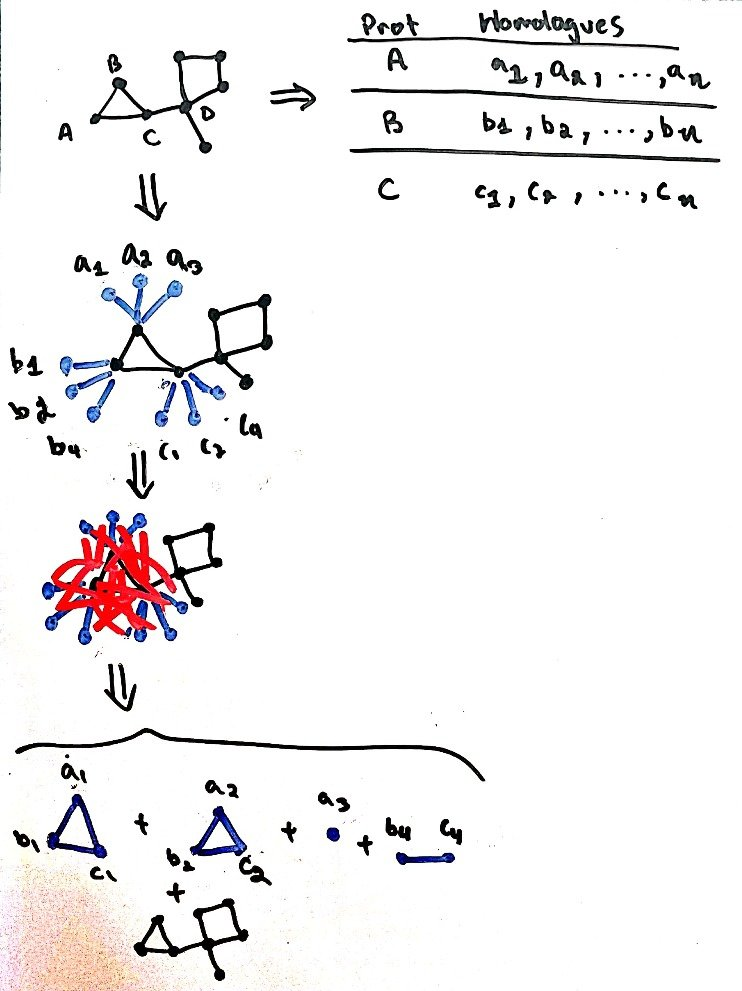
\includegraphics[width=0.45\textwidth]{images/algo_1.jpg}
    \end{center}
    \caption{Algorithm 1 for homologous network reconstruction.}
    \label{fig:algo1}
\end{figure}

\subsection{Algorithm 2: Evolutionary distance inference}

Another algorithm for evolutionary history reconstruction for proteins in a network is shown in figure ~\ref{fig:algo2}:

\begin{enumerate}
    \item Create a new edgeless network with all proteins in the PPI.
    \item For all pairs of proteins in this network,
    \begin{enumerate}
        \item If \(\texttt{\% overlap} \ge \omega_{crit}\), draw an edge between the two proteins.
    \end{enumerate}
\end{enumerate}

\begin{figure}
    \begin{center}
        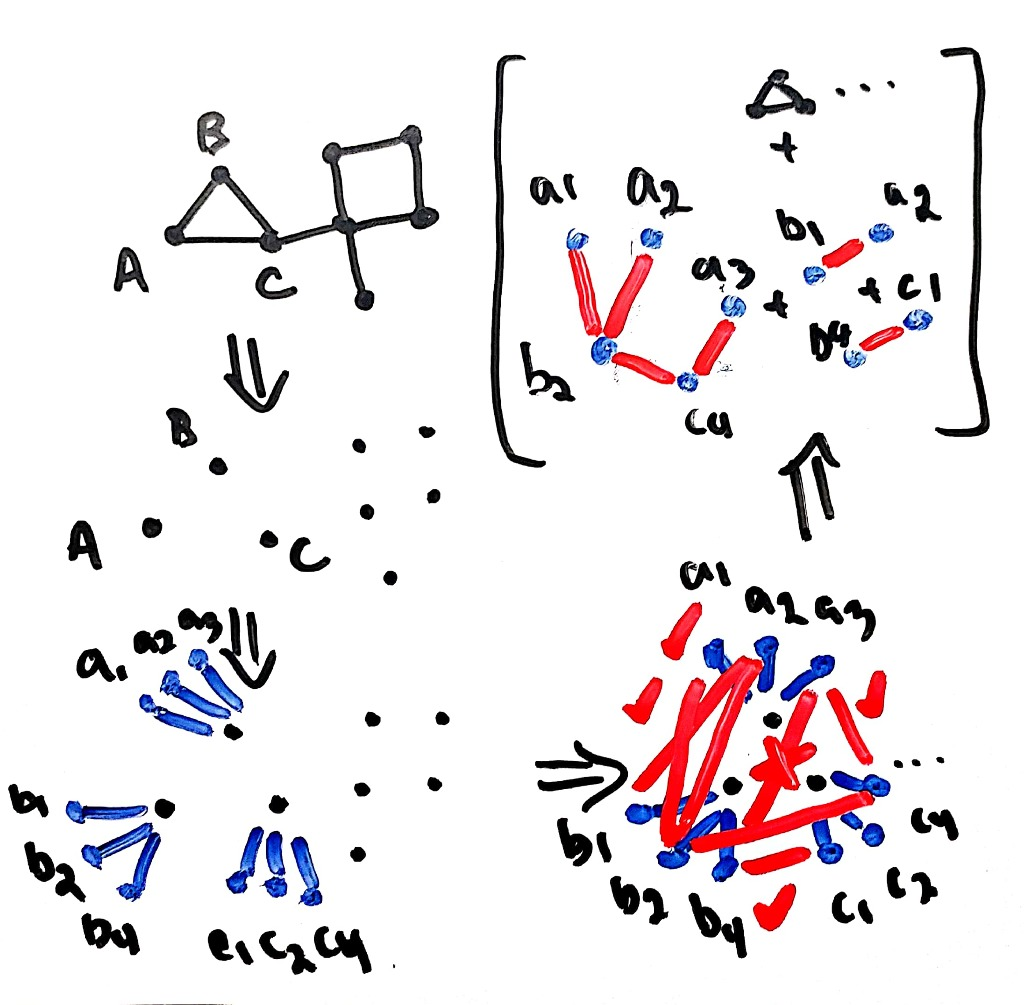
\includegraphics[width=0.45\textwidth]{images/algo_2.jpg}
    \end{center}
    \caption{Algorithm 2 for evolutionary historical network construction from homology.}
    \label{fig:algo2}
\end{figure}

\begin{equation}
    \texttt{\% overlap} = \frac{\texttt{\# shared homologs}}{\texttt{average \# of homologs between each}}
\end{equation}

\section{Evaluation}
\label{sec:evaluation}
To evaluate these algorithms, they will be tested initially on subsets, and eventually perhaps the entire, human protein-protein interaction network.

Algorithm 1 is predicted to be the more computationally-intensive algorithm of the two, so it will be first run on, say, 100 proteins of highest degree in the human PPI. If an appropriate value of the critical value \(\alpha\) is determined, this algorithm should, in principle, construct several networks, one from each species who has at least one protein that is highly homologous to at least one protein in the human PPI. The degree distribution across all of the produced networks is estimated to be fit by a power law, depending on evolutionary relationship to human proteins. Thus, this algorithm should construct a few networks closely related to humans that are fleshed-out in detail, and a great number of networks with a small number of nodes. This distribution depends entirely on evolutionary distance from human proteins. Of those ``high-degree'' networks this algorithm predicts (the "predicted network"), the predicted network is likely to be at least slightly different from the actual protein-protein interaction network. However, the level of difference between the actual and predicted (or expected; based on the null hypothesis that the two networks are not significantly different) networks can likely be quantified to understand network dynamics over evolutionary time. These data may be unavailable, however, which would preclude this analysis. The high-degree generated networks will also be analyzed for scale-free structural adherence, the list of highest-degree nodes will be compared, the network radius will be compared, perhaps along with several other metrics.

Algorithm 2 is predicted to be far less computationally-intensive because it involves a single calculation to determine whether an edge should be constructed between two "cousin" homologues. This algorithm generates possible evolutionary paths between two homologous proteins in the same or different species. Thus, one would expect that two closely-related proteins within the human protein-protein interactome, such as the globins hemoglobin and myoglobin, which are hypothesized to have arisen from gene duplication, should appear with a short evolutionary closest-path, while unrelated proteins would show an evolutionary long closest-path. Distances may be evaluated by exponentiating the distance, because relatedness would decrease exponentially with this definition of evolutionary distance. To evaluate this algorithm, the aforementioned comparisons may be made and presented in a subsequent report.

\section{Conclusion}
\label{sec:conclusion}
Homologous network inference may be useful in analyzing the relatedness of network structure across the domains of life. Algorithm 1 (figure ~\ref{fig:algo1}) provides insight into the evolution of biological networks by providing a network as a null hypothesis for protein-protein interaction network structure and evolution. This is accomplished by comparing predicted and actual protein-protein interaction networks via several network metrics. Further, algorithm 2 (figure ~\ref{fig:algo2}) provides the ability to analyze the evolutionary distance between any two proteins in the human protein-protein interactome. Moving beyond this dataset, algorithm 1 may be applied to other networks, such as transcription factor-gene networks, to illuminate differences in the evolution of transcription factor function. Leveraging algorithm 2 would here illuminate possible paths of evolution between the transcription factors.

%\fontsize{8pt}{8pt}\selectfont
%\itemsep 0.0in
%\parskip 0.03in
%\parsep 2pt


\bibliographystyle{acmsiggraph}
\nocite{*}
\bibliography{symmetry}
\end{document}
